\documentclass[border=10pt]{standalone}
\usepackage{tkz-euclide}

\usepackage{tikz}
\usetikzlibrary{calc,
                intersections,
                arrows.meta
                }

\begin{document}

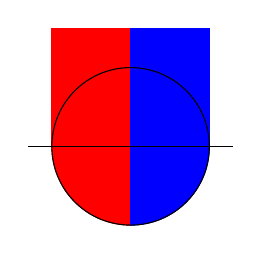
\begin{tikzpicture}
    \draw[fill=red, color=red] (0,0) rectangle (1,1.5);
    \draw[fill=blue, color=blue] (1,0) rectangle (2,1.5);
    \filldraw[fill=red, draw=red] (0,0) arc[start angle=180, end angle=270,
    radius=1] -- (1,0) -- (0,0) -- cycle;
    \filldraw[fill=blue, draw=blue] (1,-1) arc[start angle=270, end angle=360,
    radius=1] -- (1,0) -- (1,-1) -- cycle;

    \draw[thin] (-.3,0) -- (2.3,0);
    \draw[thin] (1,0) circle (1);
\end{tikzpicture}

\end{document}